\chapter{中間発表までの主な活動}

\section{ブレインストーミング}
まず各々がこのチームで開発したいアイディアを,Miro\footnote{https://miro.com/ja/}を使用して,書き出していった.

各々違う色の付箋を使用し,KJ法を使用し意見をまとめた.この活動ではさまざまな意見が挙げられたが,一番チームの共感を得たバスについて,今後の活動を絞った.

\begin{figure}[htbp]
    \centering
    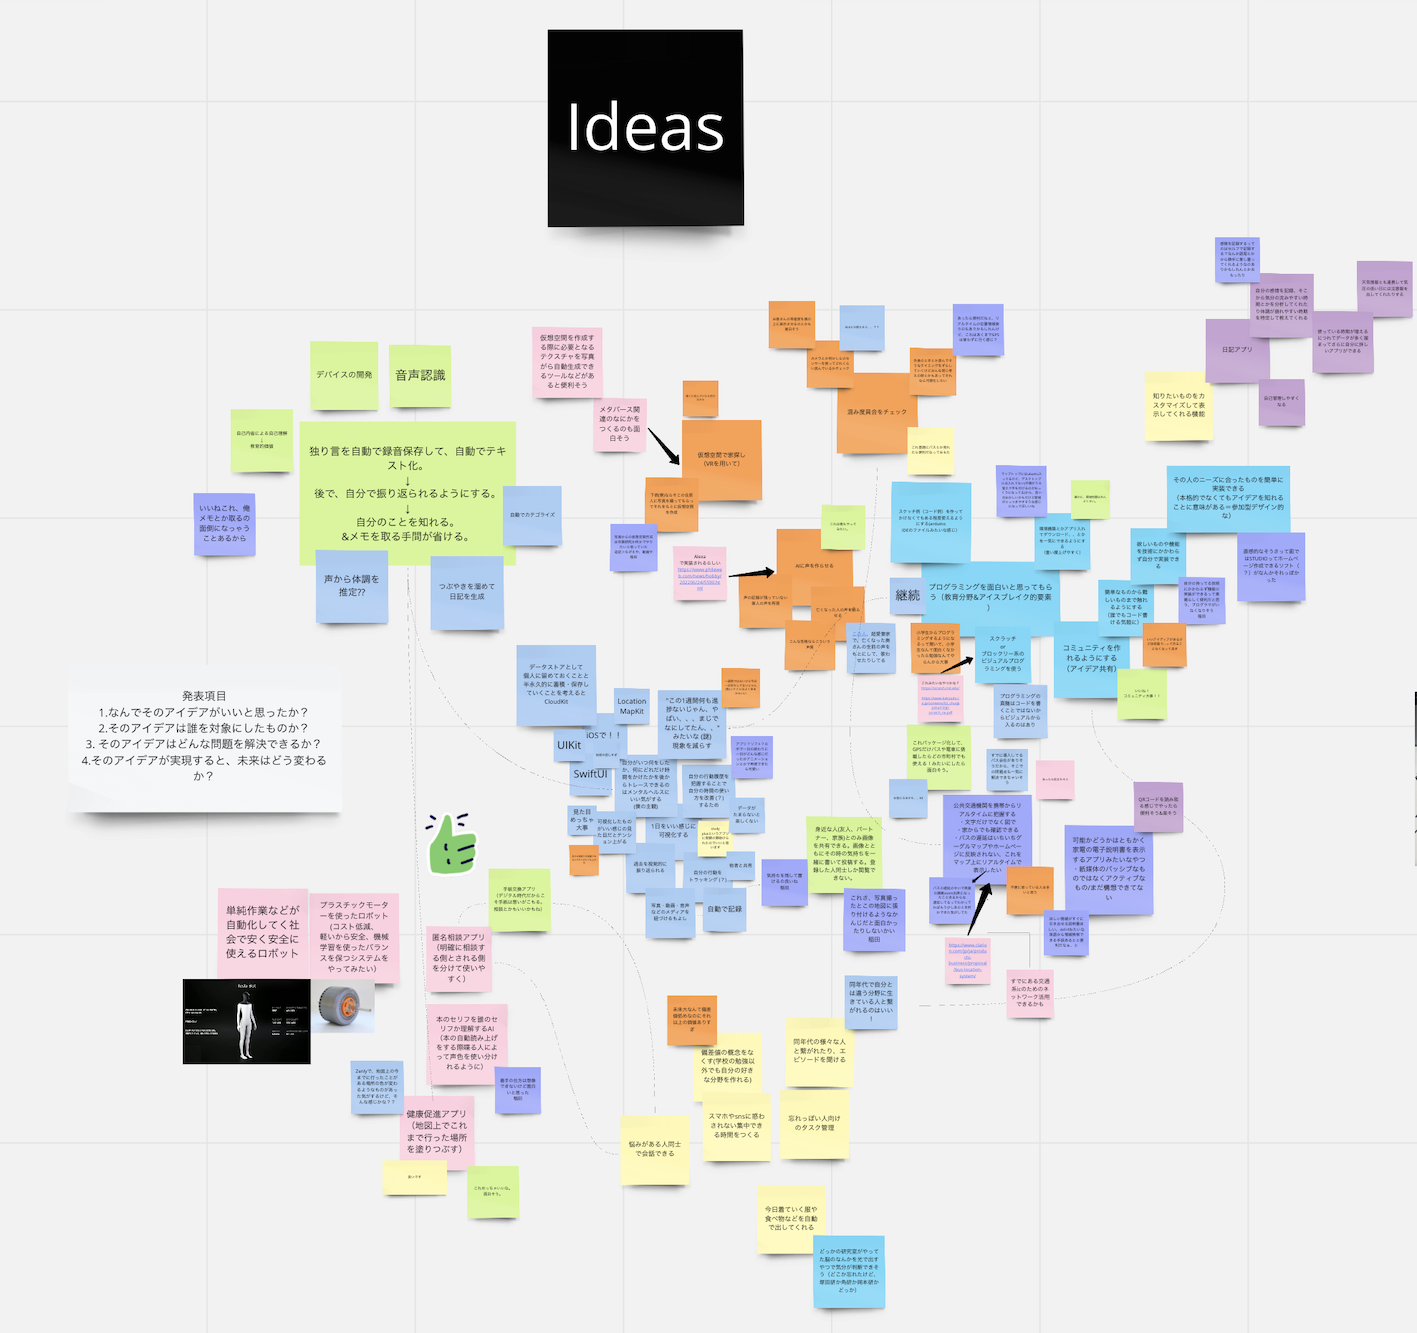
\includegraphics[width=12cm]{images/brainstorm.png}
    \caption{ブレインストーミング}
    \label{fig:brainstorm}
\end{figure}
\bunseki{大津武琉}

\section{アイディアの深掘り}

上記のブレインストーミングで挙げられたアイディアは煩雑なものであったため,実際に我々がバスを利用してきた中で不便に感じたことを考え,欲しい機能を列挙していった.

\begin{figure}[htbp]
    \centering
    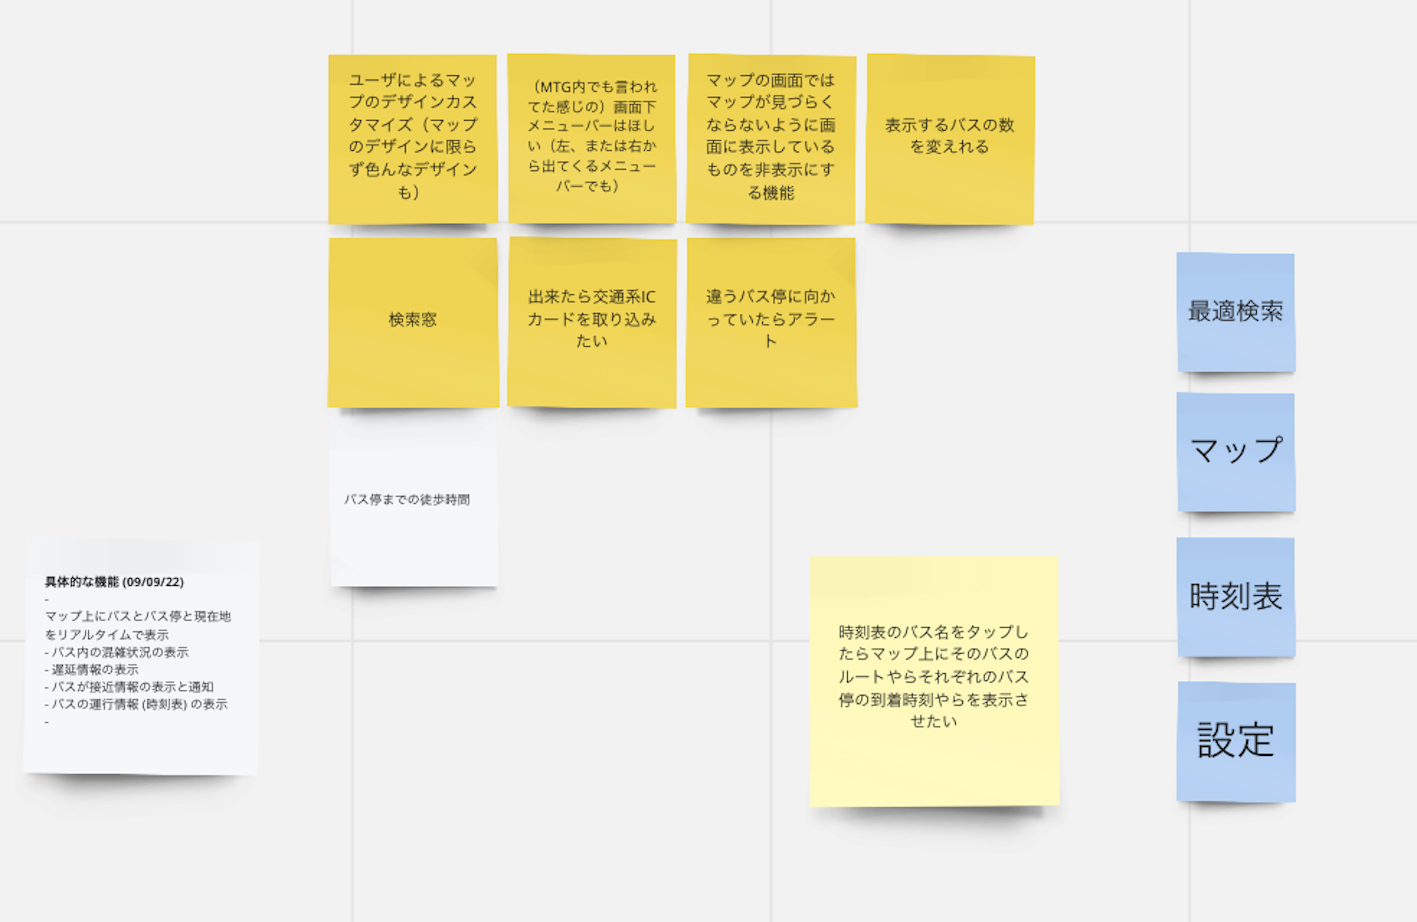
\includegraphics[width=12cm]{images/dig.png}
    \caption{アイディアの深掘り}
    \label{fig:dig}
\end{figure}

\bunseki{大津武琉}

\section{開発プラットフォームの決定}
まず,iOSとAndroidの2プラットフォームのネイティブアプリを並行して開発するか,クロスプラットフォームのネイティブアプリを開発するか,ということについて考えた.本グループの規模や技術力からクロスプラットフォーム開発に決定した.使うフレームワークとしてはFlutter\footnote{https://flutter.dev/}となった.
\bunseki{大津武琉}

\section{メンバーの役割決定}
本グループでは5人のメンバーで行っている.各メンバーの役割については以下の通りとなっている.

\subsection{プロダクトオーナー}
\begin{quote}
    \begin{itemize}
        \item 及川 寛太
    \end{itemize}
\end{quote}

\subsection{スクラムマスター}
\begin{quote}
    \begin{itemize}
        \item 大津 武琉
    \end{itemize}
\end{quote}

\subsection{デザイン}
\begin{quote}
    \begin{itemize}
        \item 下村 蒔里萌
    \end{itemize}
\end{quote}

\subsection{iOSアプリ}
\begin{quote}
    \begin{itemize}
        \item 及川 寛太
        \item 下村 蒔里萌
    \end{itemize}
\end{quote}

\subsection{Androidアプリ}
\begin{quote}
    \begin{itemize}
        \item 大津 武琉
        \item 稲田敬介
        \item ディオガーディディラン基暉
    \end{itemize}
\end{quote}

\subsection{サーバ}
\begin{quote}
    \begin{itemize}
        \item 及川 寛太
        \item 大津 武琉
    \end{itemize}
\end{quote}
\bunseki{大津武琉}

\section{Git・GitHubの習得}
チーム開発を進める中で必要不可欠であるバージョン管理アプリのGitHub\footnote{https://github.com/}の勉強会を行なった.メンバーの過半数がGitHubを触ったことがなかったため,使用経験がある人から基本的な使用方法を教えてもらい,実際にGit\footnote{https://git-scm.com/}の機能であるClone,Commit,Push,Fetch,Merge,Pullを行なってGitHubについて学んだ.
\bunseki{大津武琉}

\section{アプリ名の決定}
アプリの名前を考えることで,開発を進める上でのモチベーション維持を目指した.各々考えてきたアプリ名,キーワードを挙げていった.結果,BusとLocationを掛け合わせたBuLo(ブーロ)という名前に決定した.

\begin{figure}[htbp]
    \centering
    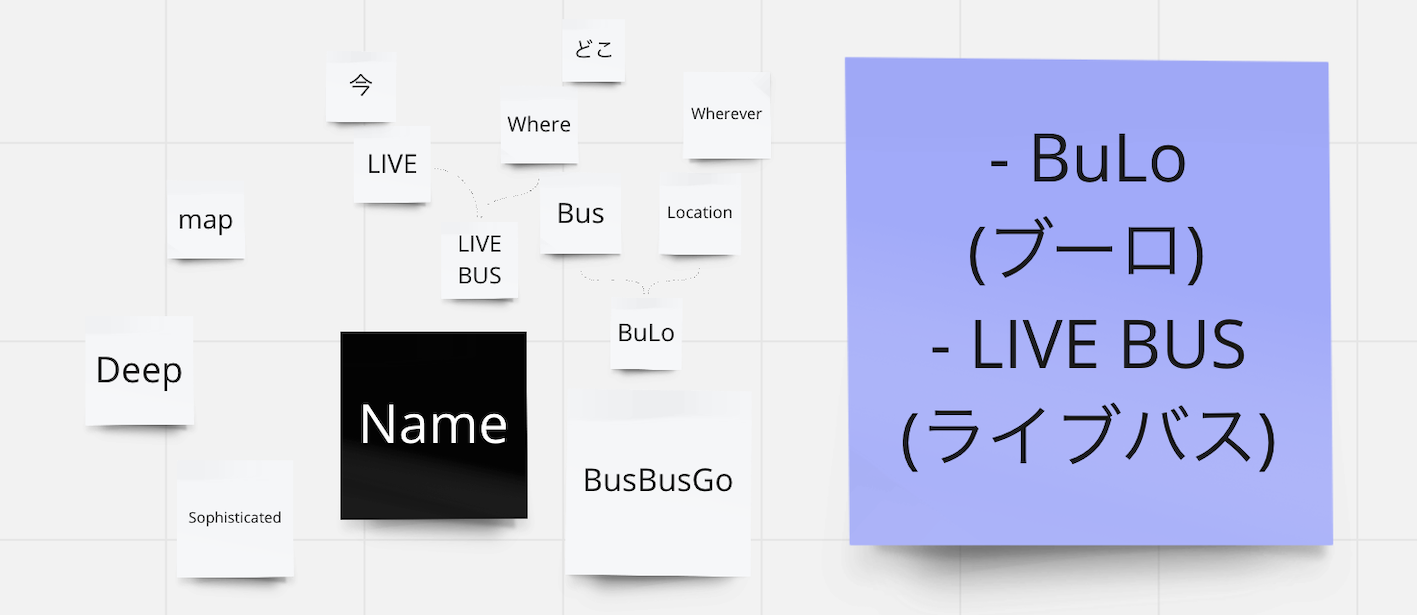
\includegraphics[width=9cm]{images/app_name.png}
    \caption{アプリ名案}
    \label{fig:app_name}
\end{figure}

\bunseki{大津武琉}

\section{プロトタイプの作成}
イメージするアプリをFigmaを使用しプロトタイプへと落とし込んだ.

\begin{figure}[htbp]
    \centering
    \includegraphics[width=12cm]{images/prototype_v2.png}
    \caption{プロトタイプ}
    \label{fig:prototype_v2}
\end{figure}

\subsection{フィードバック}
実際にプロジェクトメンバーにFigma\footnote{https://www.figma.com/}で作成した上記のプロトタイプを使用してもらった.その際たくさんの質問,指摘,意見をいただいた.「バスと人との位置関係のグラフはいるのか?」,「現在動いているバスの位置情報と自分の位置情報が分かれば大体どれくらいにバス停にいけばいいのかわかるのでは?」という意見に対し,ターゲットユーザを絞ることとした.

\subsection{ターゲットユーザ}
実際に得たフィードバックから,ターゲットユーザがしっかりと定まっておらず,このアプリは何のため,誰のためのアプリなのかがわからないことに気がついた.そこでチームでもう一度ターゲットユーザについて話し合い以下のように確立させた.

\begin{quote}
    \begin{itemize}
        \item 通勤通学にバスを使っていて,バスの乗降地点が毎回同じ
        \item バスに乗り遅れたくない
        \item バス停で待ちたくない
        \item 10代後半から20代前半
    \end{itemize}
\end{quote}

\subsection{改善}
確立させたターゲットユーザに合う機能のみを実装するとしたため,合わせてプロトタイプを改善した.

\begin{figure}[htbp]
    \centering
    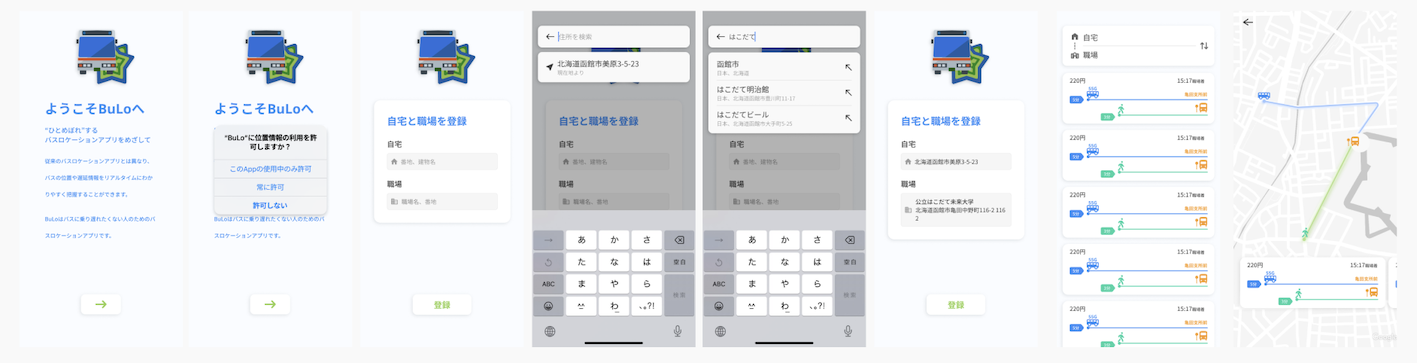
\includegraphics[width=12cm]{images/prototype_v3.png}
    \caption{フィードバックをもとに改善したプロトタイプ}
    \label{fig:prototype_v3}
\end{figure}
\bunseki{大津武琉}

\section{函館バス株式会社への訪問}
函館バス株式会社は,バス運行に関するデータを公開していないため,本グループが開発しているアプリの紹介と,データを使用させていただくために,函館バス株式会社に訪問した.そこで函館バス株式会社の方から「新しい観点からの機能でいい」というお言葉をいただき,データの使用の許可をいただいた.

\begin{figure}[htbp]
    \centering
    \includegraphics[width=12cm]{images/hakodate_bus.png}
    \caption{函館バス株式会社訪問時の様子}
    \label{fig:hakodate_bus}
\end{figure}
\bunseki{大津武琉}

\section{中間発表}
\subsection{中間発表資料の作成}
7月7日に行われる中間発表会に向けてスライド,メインポスター,サブポスターを作成した.これらの資料に関して教員に繰り返しレビューをしていただき,より伝わりやすいものへと改良を重ねた.

\subsection{中間発表会}
7月7日 (金) に発表会は行われた.そこで様々な質問や意見をいただいた.「首都圏と函館で同じ状況を想定して良いのか?」「独自性を掲げているが,(見られるのは) UIについての独自性のみで,機能についての独自性がみられない」という指摘をいただいた.これらの意見は,ターゲットユーザを絞り,合わせて実装する機能を絞った結果であると考えているため,次期バージョンにていただいた指摘をもとに改善を行う.

\begin{figure}[htbp]
    \centering
    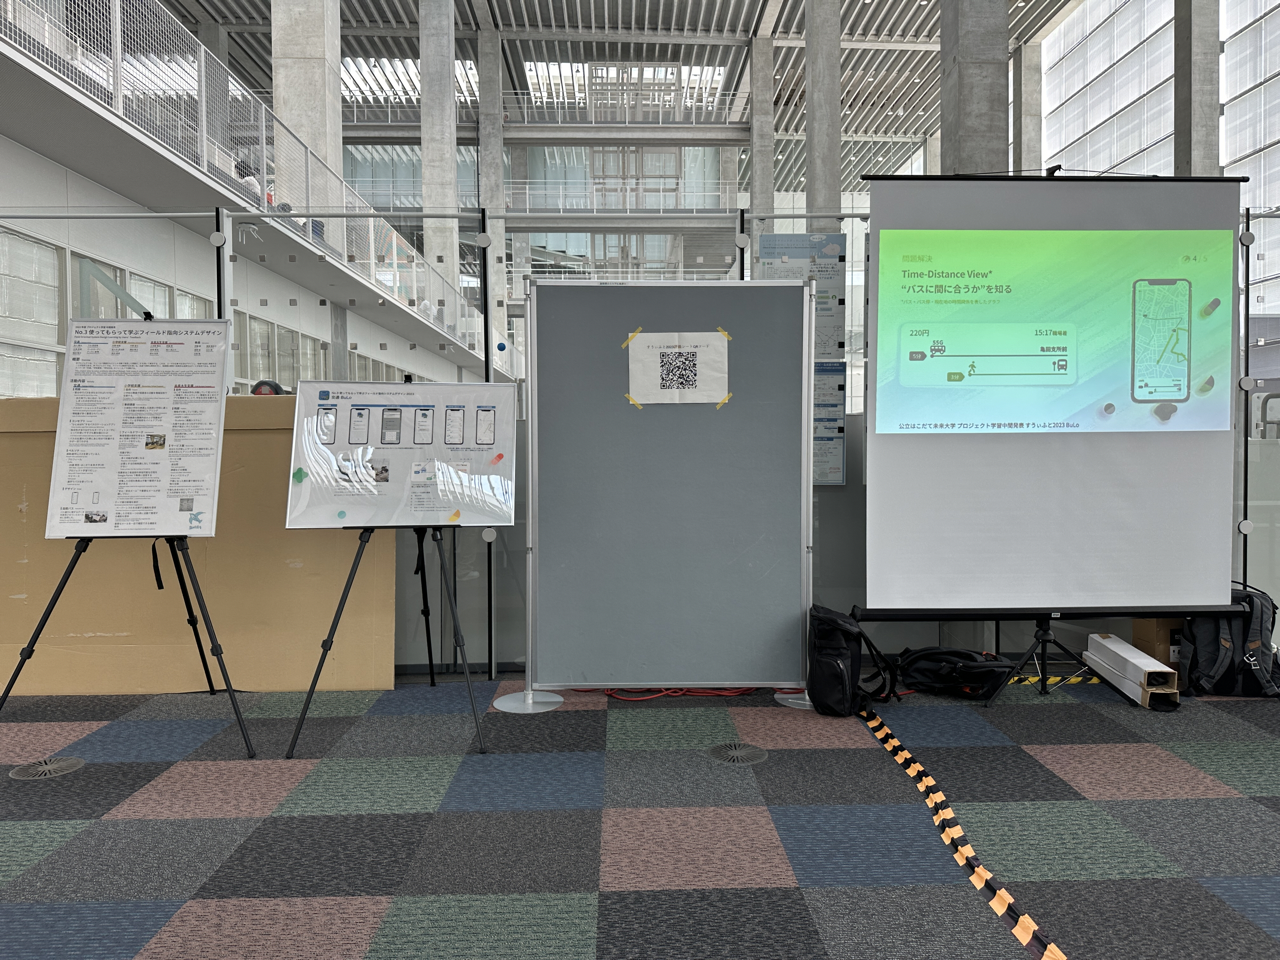
\includegraphics[width=12cm]{images/mid_presentation.png}
    \caption{中間発表会の様子}
    \label{fig:mid_presentation}
\end{figure}
\bunseki{大津武琉}
